今、このような状況にいると仮定します。あなたは長方形というstructを定義してこの面積を求めようとしています。我々の一般的な思考回路に基づけば下のような方法で実現するでしょう。


\begin{lstlisting}[numbers=none]
package main
import "fmt"

type Rectangle struct {
    width, height float64
}

func area(r Rectangle) float64 {
    return r.width*r.height
}

func main() {
    r1 := Rectangle{12, 2}
    r2 := Rectangle{9, 4}
    fmt.Println("Area of r1 is: ", area(r1))
    fmt.Println("Area of r2 is: ", area(r2))
}
\end{lstlisting}

このコードは長方形の面積を求めることができますが、area()はRectangleの(一般的なオブジェクト指向でいうような)メソッドで実現されたものではありません。Rectangleのオブジェクト(ここではr1,r2)を引数に面積を計算する関数に渡しているだけです。

このように実現してももちろん構わないのですが、図形が増えてきて、正方形、五角形ついには多角形になってきた頃、これらの面積も求めようとするとどうでしょう?この場合関数を増やすしかなくなってしまいます。関数名はそれぞれ用意しなければなりません。\texttt{area\_rectangle}, \texttt{area\_circle}, \texttt{area\_triangle}...といった具合に。

下の図で示すように、楕円が関数を表しています。これらの関数はstructに属していない(オブジェクト指向用語で言い換えるとclassに属していない)ので、structの外側に単独で存在しており、概念上どのstructにも属していないことになります。

\begin{figure}[H]
  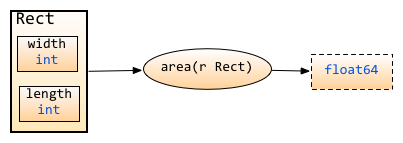
\includegraphics[width=8cm]{2.5.rect_func_without_receiver.png}
   \label{図2.8}
   \caption{メソッドとstructの関係図}
\end{figure}

明らかにこのような実現方法はエレガントではありません。それに概念からしても"面積"は"形状"の一属性です。これはある特定の形状に属しています。長方形の縦と横と同じようなものです。

このような理由から\texttt{method}の概念が生まれました。\texttt{method}はある型に属しています。この文法と関数の宣言の文法はほとんど同じです。ただ、\texttt{func}の後にreceiver(methodがくっついているということです)を追加します。

上で述べた形状の例からすると、method \texttt{area()} はある形状(たとえばRectangle)に由来して発生しています。Rectangle.area()の主語はRectangle、area()はRectangleに属するメソッドで外側の関数ではありません。

より具体的に述べると、Rectangleにはフィールドlengthとwidthが存在します。同時にarea()メソッドが存在します。これらのフィールドとメソッドは共にRectangleに属しています。

Rob Pikeの言葉を借りると:

\begin{quote}
"A method is a function with an implicit first argument, called a receiver."
\end{quote}

methodの文法は以下のとおりです:

\begin{lstlisting}[numbers=none]
func (r ReceiverType) funcName(parameters) (results)
\end{lstlisting}

はじめの例をとってmethodを実現してみます:

\begin{lstlisting}[numbers=none]
package main
import (
    "fmt"
    "math"
)

type Rectangle struct {
    width, height float64
}

type Circle struct {
    radius float64
}

func (r Rectangle) area() float64 {
    return r.width*r.height
}

func (c Circle) area() float64 {
    return c.radius * c.radius * math.Pi
}


func main() {
    r1 := Rectangle{12, 2}
    r2 := Rectangle{9, 4}
    c1 := Circle{10}
    c2 := Circle{25}

    fmt.Println("Area of r1 is: ", r1.area())
    fmt.Println("Area of r2 is: ", r2.area())
    fmt.Println("Area of c1 is: ", c1.area())
    fmt.Println("Area of c2 is: ", c2.area())
}
\end{lstlisting}

methodを使う時にはいくつか注意が必要です。

\begin{itemize}
  \item methodはまったく同じ名前でもレシーバが異なればmethodも異なります。
  \item methodはレシーバのフィールドにアクセスすることができます。
  \item methodの呼び出しは\texttt{.}を通じて行います。structがフィールドにアクセスするのと同じです。
\end{itemize}

図解:

\begin{figure}[H]
  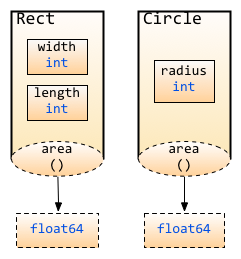
\includegraphics[width=6cm]{2.5.shapes_func_with_receiver_cp.png}
   \label{図2.9}
   \caption{異なるstructのmethodは異なる。}
\end{figure}

上の例では method area() はそれぞれRectangleとCircleに属します。この時これらの Receiver は Rectangle と Circleになります。またはこのarea()メソッドはRectangle/Circleを主語とします。

\begin{quote}
特に、図中のmethodは破線で表示しています。これは、このメソッドのレシーバは値渡しであり、参照渡しではありません。そうです。レシーバはポインタでもいいのです。両者の違いはポインタはレシーバがエンティティの内容に操作を行うことがあるのに対し、普通の型ではレシーバは操作するオブジェクトのコピーでしかありません。オリジナルのエンティティに対して操作が発生しないのです。詳細は後述します。
\end{quote}

methodはstructの上でしか使用されないのでしょうか?当然違います。これはカスタム定義型、ビルトイン型、structなどあらゆる型でも定義することができます。ちょっとよくわからなくなってきましたか?何がカスタム定義型だ、カスタム定義型はstructじゃないのか。そういうわけではありません。structはカスタム定義型のなかでも比較的特殊な型であるだけです。下のような宣言で実現します。

\begin{lstlisting}[numbers=none]
type typeName typeLiteral
\end{lstlisting}

以下のカスタム定義型の宣言のコードをご覧ください。

\begin{lstlisting}[numbers=none]
type ages int

type money float32

type months map[string]int

m := months {
    "January":31,
    "February":28,
    ...
    "December":31,
}
\end{lstlisting}

わかりましたか?簡単でしょう?このように自分のコードの中に意味のある型を定義することができるのです。実際はエイリアスを定義しているだけです。Cのtypedefに似たようなもので、例えば上のagesはintの代わりになっています。

それじゃあ、\texttt{method}にもどりましょう。

カスタム定義型の中で任意の\texttt{method}を定義することができます。次にちょっと複雑な例を見てみましょう。

\begin{lstlisting}[numbers=none]
package main
import "fmt"

const(
    WHITE = iota
    BLACK
    BLUE
    RED
    YELLOW
)

type Color byte

type Box struct {
    width, height, depth float64
    color Color
}

type BoxList []Box //a slice of boxes

func (b Box) Volume() float64 {
    return b.width * b.height * b.depth
}

func (b *Box) SetColor(c Color) {
    b.color = c
}

func (bl BoxList) BiggestColor() Color {
    v := 0.00
    k := Color(WHITE)
    for _, b := range bl {
        if bv := b.Volume(); bv > v {
            v = bv
            k = b.color
        }
    }
    return k
}

func (bl BoxList) PaintItBlack() {
    for i, _ := range bl {
        bl[i].SetColor(BLACK)
    }
}

func (c Color) String() string {
    strings := []string {"WHITE", "BLACK",
                         "BLUE", "RED", "YELLOW"}
    return strings[c]
}

func main() {
    boxes := BoxList {
        Box{4, 4, 4, RED},
        Box{10, 10, 1, YELLOW},
        Box{1, 1, 20, BLACK},
        Box{10, 10, 1, BLUE},
        Box{10, 30, 1, WHITE},
        Box{20, 20, 20, YELLOW},
    }

    fmt.Printf("We have %d boxes in our set\n",
               len(boxes))
    fmt.Println("The volume of the first one is",
                boxes[0].Volume(), "cm³")
    fmt.Println("The color of the last one is",
                boxes[len(boxes)-1].color.String())
    fmt.Println("The biggest one is",
                boxes.BiggestColor().String())

    fmt.Println("Let's paint them all black")
                boxes.PaintItBlack()
    fmt.Println("The color of the second one is",
                 boxes[1].color.String())

    fmt.Println("Obviously, now, the biggest one is",
                boxes.BiggestColor().String())
}
\end{lstlisting}

上のコードはconstでいくつかの定数を定義しています。その後カスタム定義型を定義しています。

\begin{itemize}
  \item Colorはbyteのエイリアスです。
  \item struct:Boxを定義します。3つの縦横高さのフィールドと色プロパティを持っています。
  \item slice:BoxListを定義します。Boxを持っています。
\end{itemize}

次に上のカスタム定義型をレシーバとしてmethodを定義します。

\begin{itemize}
  \item Volume()はレシーバをBoxとして定義します。Boxの体積を返します。
  \item SetColor(c Color)はBoxの色をcに変更します。
  \item BiggestColor()はBoxListに定義されており、listの中の体積が最大の色を返します。
  \item PaintItBlack()はBoxListのすべてのBoxの色を全部黒に変更します。
  \item String()はColorに定義されており、Colorの具体的な色を返します(文字列形式)
\end{itemize}

上のコードは文字で書くと非常に簡単に思えませんか?私達は問題を解決する場合問題の描写を通して、対応するコードを書くことで実現します。


